\section*{Summary}
\begin{markdown}

## Background

The focus of our team's work is on using explainable machine learning, clinical pathway simulation, and geographic modelling, applied to national clinical audit data to identify between-hospital variation in clinical processes and decision-making, and to understand the impact of that variation on patients. Our work is mostly in collaboration with the Sentinel National Stroke Audit Programme (SSNAP), and we provide analysis to national and regional NHS organisations.

We would like to enhance our methodology by adding causal analysis methods to strengthen the conclusions our modelling and machine learning explainable machine learning. 

## Method development

As no method is perfect we wish to be able to develop a range of causal models to allow triangulation of results, and identify the best methods to incorporate into our integrated modelling and data science approach. This will allow us to propose and refine causal structures for discussion with clinicians. We wish to investigate the following methods, and incorporate a mix of them into our analysis.

* Target trial emulation
* Propensity score or nearest-neighbour matching
* Inverse probability weighting
* Instrumental variable analysis
* Pearline causal analysis framework


## Research questions

This enhanced methodology has potential immediate uses, in coordination with existing NIHR-funded projects, that will benefit patients and the NHS. Though we expect these methods to have wide range and continued application in the team's work, we will develop these methods around central research questions, based on analysing more than 300,000 patient records in SSNAP. These questions align with currently funded work that will inform organisation and delivery of specialist stroke services.

Background: The majority (80%) of strokes are caused by a clot in the brain (ischaemic stroke). For those patients with ischaemic stroke arriving in the first few hours after stroke onset, there is the possibility to reduce/remove the clot by use of clot-busting medication (thrombolysis) or surgery (thrombectomy). Use of thrombolysis varies very significantly between hospitals (ranging from 5% to 50% of patients who arrive in time for treatment. Overall, thrombolysis rates are 11% of stroke admissions against a NHS target of 20%. Using explainable machine learning we have demonstrated that the majority of variation between hospitals is due to differences in clinical processes and decision-making, rather than differences in local patient populations. Low use is, in part, caused by hesitancy that the risks (a 2% of serious bleed in the brain) outweigh the benefits. This can cause concern around a drive to increase of thrombolysis. Our questions therefore centre mostly on building confidence in where thrombolysis use can/should be improved.

1) Will increasing use of thrombolysis in the NHS improve patient outcomes (or at which point of use do harms outweigh benefits)?

2) What is the expected benefit and risk of harm of thrombolysis in three subgroups of patients where we have identified that there is significant between-hospital variation in use of thrombolysis?

    * Mild stroke (at presentation)
    * Presence of prior disability
    * Imprecisely known stroke onset time
   
Additionally, we have a specific question on the benefits and risks of bypassing a local stroke unit, in order to take a patient directly to a thrombectomy-capable centre. Thrombectomy has greater benefit than thrombolysis in more sever strokes, but in the pre-hopsital setting severe ischaemic strokes are not readily distinguished from haemorrhagic strokes (which will not benefit from thrombolysis or thrombectomy). Our question relates to how benefit of faster thrombectomy should be weighed against any potential harm caused by delayed hospital admission for those patients who do not benefit from thrombectomy.

3) What effect will extending ambulance travel times (in order to take more patients to specialist stroke centres offering both thrombolysis and thrombectomy) have on patients who do not receive thrombolysis or thrombectomy? Particular focus will be made on haemorrhagic stroke patients who may be easily be confused with ischaemic stroke patients who would benefit from thrombectomy?



* We are working with the national stroke audit to help build machine learning into their national audit outputs, especially on unnecessary variation in use of clot-bust treatments in stroke. We are working with NHS-England to provide this analysis to new communities of practice in stroke. We have identified that a majority of the variation comes from differences in clinical decision-making rather than in differences in local patient populations. This is a NIHR-funded project\footnote{https://fundingawards.nihr.ac.uk/award/NIHR134326}. The methodological development will enhance the breadth and depth of that work, helping to identify and isolate causal relationships. Improving use of clot-busting drugs will benefit patients (and should reduce inpatient length of stay).

* We are working on stroke projects focussing on the pre-hospital pathway\footnote{https://fundingawards.nihr.ac.uk/award/NIHR202361} and the use of mobile stroke units\footnote{https://fundingawards.nihr.ac.uk/award/NIHR153982 (page due to go live)}. The methodological development above will add value to these, and other similar, projects. For example, it has previously been assumed that outcome from hemorrhagic stroke (the 20\% of strokes that are caused by a bleed rather than a clot) is independent of ambulance travel time, but some recent clinical trials on taking stroke patients further, to a hospital with more capabilities for stokes caused by clots, have suggested this may not be true. Using methods such as clinical trial emulation and our large database of stroke data we will have the potential to enhance our pre-hospital stroke care model to better model outcomes of haemorrhagic strokes with alternative pre-hospital pathways.

During this project we will hold stakeholder workshops, to obtain feedback on the work. This will use our existing stakeholder network across the Sentinel Stroke National Audit, Integrated Stroke Delivery Networks (ISDN) and Integrated Care Systems (ICS). We will also hold regular meetings with our stroke Patient and Carer Involvement group.

In addition to development of the methodology, this project will be used to develop the skills and capabilities of Kerry Pearn (co-PI) who will lead the project with assistance from Michael Allen (Co-PI). The stroke modelling and data science team is a stable team, funded by research grants and NHS-contracted work, and the techniques and skills developed here will find long-term use and benefit.

\end{markdown}




\begin{figure}[htbp]
\centering
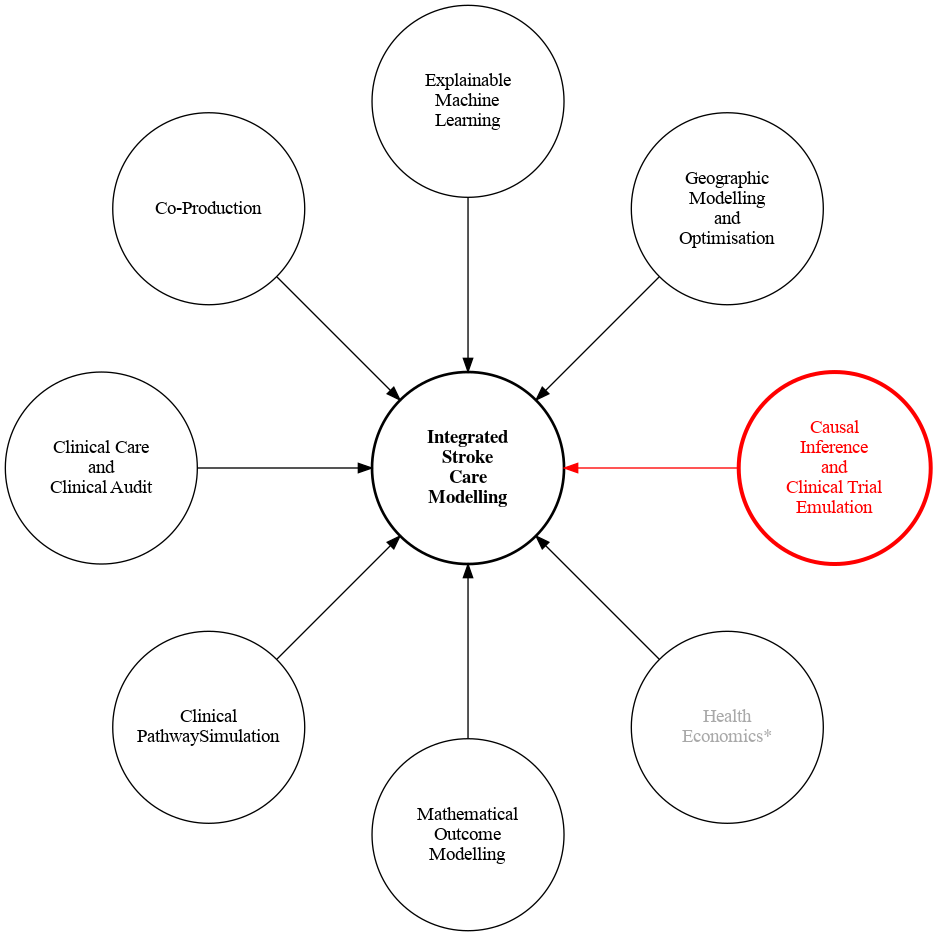
\includegraphics[width=0.6\textwidth]{./images/skills}
\caption{How planned methodology development (red) fits in with existing team skills (black) or collaborative work (grey). All methods are fully pubslished with open code.}.
\label{fig:expertise}
\end{figure}
